% !TEX program = xelatex
\documentclass[12pt]{article}

\usepackage{hyperref}
\usepackage{enumitem,graphicx}


\usepackage{amsmath,amsfonts,amssymb}
\usepackage{amsthm}
%\usepackage{bidipoem} % for poem -> traditionalpoem
%\usepackage{longtable} % for longtables

%\usepackage{pgf,tikz,pgfplots}
%\pgfplotsset{compat=1.15}
%\usepackage{mathrsfs}
%\usetikzlibrary{arrows}
%%\pagestyle{empty}


\usepackage{xepersian}
\settextfont{Yas}
\setdigitfont{Yas}



\defpersianfont\nast{IranNastaliq}
\defpersianfont\sols{XB Sols}
\defpersianfont\naz{B Nazanin}
\defpersianfont\yas{Yas}


\title{پاسخ تمرین اول پایگاه داده}
\author{محمد رضیئی فیجانی\\ 9423052}

%\newtheorem{thm}{قضیه}[section]
%\newtheorem{Def}{تعریف}[section]
%\newtheorem{test}{تمرین}
\newtheorem{question}{سوال}
%\newcommand{\dd}{\, \mathbf{d} }
\newcommand{\prd}{\triangleright\!\!\triangleleft\,}

\begin{document}
\maketitle

\section{پاسخ سوالات}\label{chpt1}
\begin{question}
	چون هر زیر مجموعه غیر تهی از k کلید کاندیدا میتواند یک ابرکلید باشد، بنابراین تعداد 
	$2^k - 1$
	ابرکلید خواهیم داشت.
\end{question}
\begin{question}
درستی و نادرستی در زیر بررسی شده است.
\begin{enumerate}
	\item
	درست است.
	
	اگر روی دو مجموعه به صورت جداگانه عمل select را انجام دهیم و سپس روی نتیجه حاصل اجتماع بگیریم پاسخ با حالتی که روی اجتماع دو جدول select کنیم، تفاوتی ندارد.
	
	\item
	نادرست است.
	
	اگر ابتدای projection انجام دهیم؛ ممکن است ستونی را که میخواهیم روی آن select کنیم، انتخاب نشده باشد. از این رو نتیجه با سمت دیگر تساوی، برابر نخواهد بود. معمولا از سمت راست تساوی استفاده می شود.
	
	\item
	درست است.
	
	دو مجموعه R  و S با یک‌دیگر اشتراکی دارند که در این قسمت، بعضی از اعضای آن شرط $\theta$ را برآورده می کنند.
	
	\item
	نادرست است.
	
	زیرا اشتراک هر دو مجموعه ای، زیرمجموعه هریک از آن‌هاست. بنابراین کلید کاندیدای M یا N می‌تواند به تنهایی به‌عنوان کلید کاندیدای $M \cap N$ باشد.
	
	\item
درست است.

وقتی از مجموعه M، تعدادی عضو کاسته شود؛ همچنان می‌توان از کلید کاندیدای قبلی استفاده کرد.
	
	\item
درست است.

چون 	در ضرب دو جدول، زوج مرتب $(m,n)$ بوجود می‌آید بطوریکه
 $m,n \in \mathbb{N} $
 ؛ برای همین هر رکورد با ترکیبی از کلید کاندیدای M و  N مشخص می‌شود و زیرمجموعه‌ای از این کلید نمی‌تواند کلید کاندیدا باشد. در نتیجه، کلید کاندیدای ضرب دو مجموعه است.
	
	
	
	
\end{enumerate}
\end{question}
\begin{question}
	پاسخ :
\begin{latin}
\begin{enumerate}[label=\alph*)]
\item

	$$
	\Pi_{\mathrm{date}}\left(\sigma_{\text{origin}=\mathrm{"Tehran"}}(\mathrm{Trip}))\right)
	$$
	
	
\item 
	\[
	\Pi_{\mathrm{dest}} \left(
	\mathrm{Trip} \prd \Pi_\mathrm{trip\_id}(\sigma_\mathrm{name\,=\,"A"}
	(
	\mathrm{Passenger}\prd \mathrm{Pass\_in\_trip}
	))
	\right)
	\]
	
	
\item 
	\[
	\Pi_{\mathrm{Pass\_id}} \left(
	\mathrm{Pass\_in\_Trip} \prd \Pi_\mathrm{trip\_id}(\sigma_\mathrm{(duration < 12)\,\wedge\,(date > 1396-06-06)}
	(
	\mathrm{Trip}
	))
	\right)
	\]
	

\end{enumerate}
\end{latin}
\end{question}

\begin{question}
	پاسخ :
%\begin{flushright}
\begin{enumerate}
	\item[.a]
	نتیجه این پرس‌و‌جو نام تمام تهیه کنندگانی است که شهر آن‌ها با تهیه‌کننده‌ای با شماره 8 یکی باشد.
		
	\item[.b]
	
	$$
	\Pi_{\mathrm{s\_id}}\left(\sigma_{\text{s\_city}=\mathrm{"Tehran"}}(\mathrm{Producer}))\right)
	$$
	
	
	\item[.c]
	\[
	\Pi_{\mathrm{s\_name}} \left(
	\mathrm{Producer} \prd \Pi_\mathrm{s\_id}(\sigma_\mathrm{p\_color\,=\,"blue"}
	(
	\mathrm{Piece}\prd \mathrm{Producer}
	))
	\right)
	\]
	
	
	\item[.d]
	\[
	\Pi_{\mathrm{s\_name}} \left(
	\sigma_\mathrm{T.s\_name\,\ne\,C.d\_name}(\rho_T( \mathrm{Producer}
	\prd \mathrm{Producer}
	)
	\times \rho_C(c.)
	)
	\right)
	\]
	
	در این پرس‌و‌جو از نتیجه قسمت قبلی سوال با همان نام استفاده شده است.
	 (c.)
	.  برای اینکه مطمئن شویم تولید کننده حداقل یک محصول تولید کرده، از natural join دو جدول Produce و Producer استفاده کرده‌ایم.
	
\end{enumerate}
%\end{flushright}
\end{question}
\begin{question}
	فایل های مورد نظر در ضمیمه آورده شده اند. همچنین دیتاها به صورت دستی وارد شده اند.
	
	همچنین با استفاده از زبان php و xampp چیزی محیطی را فراهم شده است که در  
	\href{https://github.com/mohammadraziei/DB2019/}{github}
	مربوطه، قابل دسترس است.

\begin{figure}[h!]
\begin{center}
		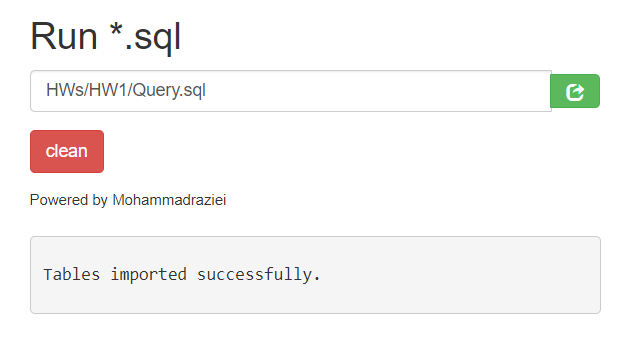
\includegraphics[height=5cm]{Run_sql.jpg}
\caption{محیط نوشته شده با php}
\end{center}
\end{figure}
\end{question}








\section{github}\label{chpt2}
تمامی فایل های تمرینات این درس در آدرس زیر در 
\href{https://github.com/mohammadraziei/DB2019/}{github}
قابل دسترسی می باشد.

\begin{latin}
\begin{center}
\href{https://github.com/MohammadRaziei/DB2019/tree/master/Workspace/HWs}{https://github.com/MohammadRaziei/DB2019/tree/master/Workspace/HWs}
\end{center}
\end{latin}



\begin{center}
\vspace{1.5cm}
\huge
پایان
\end{center}
\end{document}